\documentclass[10pt]{article}

\usepackage[a4paper,margin=1.9cm]{geometry}
\usepackage{amsmath,amssymb,booktabs,tabularx,array}
\usepackage{xcolor,tikz,fancyhdr}
\usepackage[hidelinks]{hyperref}
\usetikzlibrary{positioning}

\definecolor{ink}{HTML}{24324A}
\definecolor{rose}{HTML}{A84F70}
\definecolor{green}{HTML}{2F6B50}
\definecolor{softrose}{HTML}{F8E7ED}
\definecolor{softgreen}{HTML}{E9F2EC}
\definecolor{softblue}{HTML}{E9EDF5}
\newcommand{\eid}[1]{\textcolor{green}{\texttt{#1}}}
\newcommand{\status}[1]{\textcolor{rose}{\textbf{#1}}}
\newcolumntype{Y}{>{\raggedright\arraybackslash}X}
\newcolumntype{P}[1]{>{\raggedright\arraybackslash}p{#1}}

\pagestyle{fancy}
\fancyhf{}
\lhead{\textcolor{ink}{SPS Part 2 learning draft}}
\rhead{\textcolor{ink}{2026-07-16}}
\cfoot{\thepage}
\setlength{\headheight}{14pt}

\title{\textcolor{ink}{\textbf{Learning SPS Through Its Literature Lineage}}\\
\large A worked technical reading}
\author{Moxian Qian}
\date{Draft, 16 July 2026}

\begin{document}
\maketitle

\noindent
\colorbox{softrose}{\parbox{0.96\linewidth}{
\textbf{Draft status.} The SPS paper is mapped at equation level; comparisons
with P002, P003, and P007 are still in progress.}}

\section{Learning Question}

Which earlier methods are needed to understand SPS, how does SPS work, and
which technical differences are supported by the current sources? The target
is T3: reconstruct the ordered algorithm after explaining its core formulas.
Code mapping and reproduction are not requested.

\section{Lineage-First Route}

\begin{center}
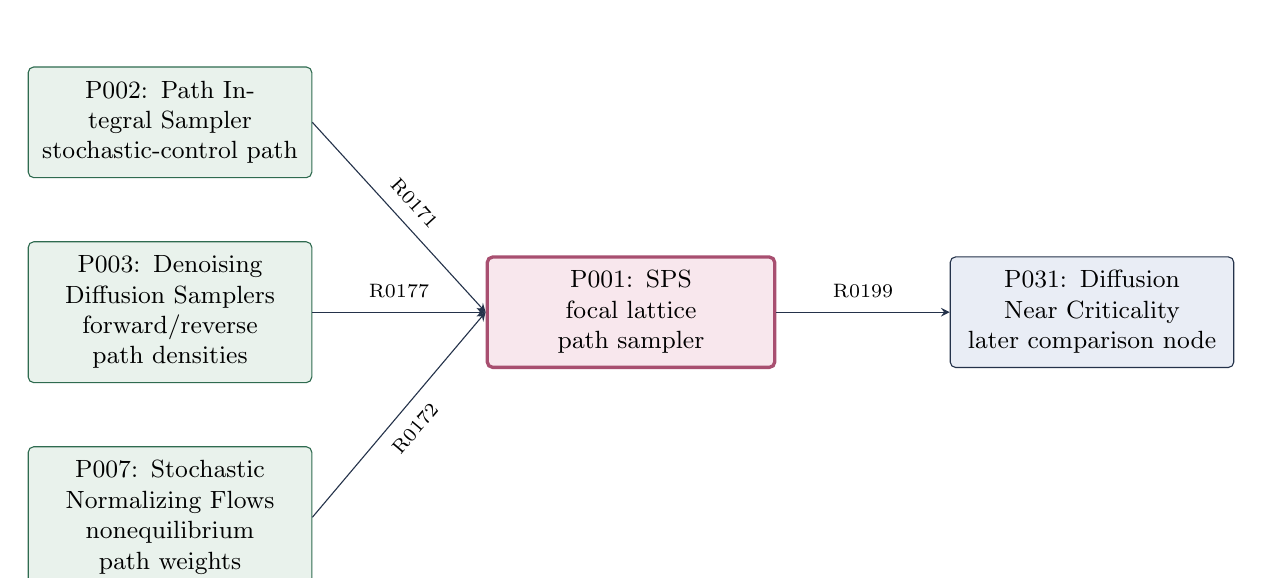
\begin{tikzpicture}[
  node distance=8mm and 10mm,
  every node/.style={font=\small,align=center,rounded corners=2pt,inner sep=5pt},
  source/.style={draw=green,fill=softgreen,text width=3.25cm},
  focal/.style={draw=rose,fill=softrose,line width=1.2pt,text width=3.3cm},
  later/.style={draw=ink,fill=softblue,text width=3.25cm},
  arrow/.style={->,>=stealth,draw=ink}
]
\node[source] (p002) {P002: Path Integral Sampler\\stochastic-control path};
\node[source,below=of p002] (p003) {P003: Denoising Diffusion Samplers\\forward/reverse path densities};
\node[source,below=of p003] (p007) {P007: Stochastic Normalizing Flows\\nonequilibrium path weights};
\node[focal,right=22mm of p003] (p001) {P001: SPS\\focal lattice path sampler};
\node[later,right=22mm of p001] (p031) {P031: Diffusion Near Criticality\\later comparison node};
\draw[arrow] (p002.east) -- node[above,sloped,font=\scriptsize] {R0171} (p001.west);
\draw[arrow] (p003.east) -- node[above,font=\scriptsize] {R0177} (p001.west);
\draw[arrow] (p007.east) -- node[below,sloped,font=\scriptsize] {R0172} (p001.west);
\draw[arrow] (p001.east) -- node[above,font=\scriptsize] {R0199} (p031.west);
\end{tikzpicture}
\end{center}

\noindent\textbf{Edge meaning.} R0171, R0172, R0177, and R0199 are checked
direct-citation relations. Dijkstra costs set the reading order; the technical
claims use the cited source sections.

\section{Finding The Technical Difference}

\begin{tabularx}{\linewidth}{@{}p{1.05cm}Y Y@{}}
\toprule
Step & Read first & Purpose \\
\midrule
I0 & exact P001 version and source hash & lock the object \\
I1 & contribution paragraph and overview & record the authors' claimed delta \\
I2 & matching P002/P003/P007 equations & subtract inherited components \\
I3 & P001 Eqs. (2.2)--(2.19) & isolate the operative mechanism change \\
I4 & P001 Tables 1--4 and Fig. 8 & ask which evidence isolates the change \\
I5 & P031 method and direct-citation context & test persistence without inferring adoption \\
\bottomrule
\end{tabularx}

\medskip
The current candidates are the paired forward/backward Langevin
parameterization, the path-space log-ratio objective, and full-trajectory IMH.
These mechanisms appear in P001, but their novelty rank remains
\status{pending} until the predecessor equations are aligned.

\section{Technical Mechanism}

\begin{enumerate}
\item Sample the initial field from a tractable prior.
\item Generate a forward Langevin path with a learned drift
  (P001 p.~5, Eq.~(2.2), \eid{E-260613790-M}).
\item Evaluate an auxiliary backward path on the same trajectory
  (P001 pp.~5--6, Eqs.~(2.3), (2.7)--(2.8)).
  Evidence: \eid{E-260613790-M}.
\item Minimize the expected forward/backward path log-ratio
  (P001 p.~6, Eq.~(2.13), \eid{E-260613790-M}).
\item Propose independent full trajectories and apply trajectory-level IMH
  (P001 pp.~7--9, Eqs.~(2.18)--(2.19), \eid{E-260613790-M}).
\item Estimate observables and autocorrelation from the corrected chain.
\end{enumerate}

\section{Core Formulas And Limits}

\begin{align}
s_{i+1} &= s_i+\sigma_\theta^2(t_i)K_{\theta,F}(s_i,t_i)\Delta t
 +\sigma_\theta(t_i)\xi_i\sqrt{\Delta t}, \tag{F01}\\
D_{\mathrm{KL}} &= \int dq_F(\tau)\log\!\frac{dq_F(\tau)}{d\widetilde q_B(\tau)}, \tag{F02}\\
P_{\mathrm{acc}} &= \min\!\left(1,
\frac{\widetilde\pi^*(s_T')T(s_T'\!\to s_T)}
{\widetilde\pi^*(s_T)T(s_T\!\to s_T')}\right). \tag{F03}
\end{align}

F01 generates the path, F02 trains it without the target normalization
constant, and F03 corrects a support-covering proposal. Finite model capacity,
training, and discretization leave residual irreversibility before correction
(P001 pp.~7--8, \eid{E-260613790-L}).

\section{Evidence And Technical Review}

\begin{tabularx}{\linewidth}{@{}P{2.5cm}Y P{3.5cm}@{}}
\toprule
Claim & What the source supports & Limit \\
\midrule
Corrected observables & Agreement with the reported HMC values in the tested
2D $L\times 8$ scan (P001 Figs.~3--5, Tables~1--3,
\eid{E-260613790-R}) & benchmark-specific \\
Autocorrelation & About 0.5 for SPS+IMH and about 160 for HMC in the reported
$L=64$, $\kappa=0.27$ comparison (P001 Fig.~8,
\eid{E-260613790-R}) & different update units; not a cost ratio \\
Timing & About 1.1--1.2 h training and 1.1--2.1 min generation across the
reported sizes (P001 Table~4, \eid{E-260613790-L}) & no matched HMC GPU-hour comparison \\
Exactness & trajectory-level IMH restores target invariance
(\eid{E-260613790-M}) & requires target-support coverage \\
\bottomrule
\end{tabularx}

\section{Learning Status}

\begin{tabularx}{\linewidth}{@{}P{1cm}Y P{2.4cm}@{}}
\toprule
Level & Evidence & Status \\
\midrule
T0 & exact version, URL, hash, and identity rows & pass \\
T1 & explanation preserving result and cost limits & pass \\
T2 & F01--F04 with symbols, roles, assumptions, and anchors & pass \\
T3 & focal algorithm plus predecessor comparison & \status{pending} \\
T4 & official equation-to-code mapping & not requested \\
T5 & minimal reproduction & not requested \\
\bottomrule
\end{tabularx}

\medskip
\noindent\textbf{Next action.} Upgrade P002, P003, and P007 to detailed R0--R6
records; align their path objectives and correction rules with P001; then update
the innovation table and technical review. The current conclusion covers the
paired-path lattice mechanism and its trajectory-level correction; novelty and
cost comparisons remain open.

\end{document}
